\documentclass[final,hyperref={pdfpagelabels=false}]{beamer}

\usepackage{graphics, subfigure}
\usepackage{color}
\usepackage[english]{babel}
\usepackage[orientation=portrait,size=a0,scale=1.4]{beamerposter}
\usepackage{fp}% http://ctan.org/pkg/fp
\usepackage{wrapfig} % wrap text around figures
\usepackage{calc} % easy adding dimensions
\usepackage[export]{adjustbox} % left, right-align includegraphics
\newlength{\columnheight}
\setlength{\columnheight}{98cm}
\def\marginwidthratio{0.08}
\FPeval{\contentwidthratio}{1-\marginwidthratio}
\FPeval{\tightcontentwidthratio}{1-(\marginwidthratio / 2)}
\def\insidecolumnsinter{0.05}

\graphicspath{{figures/}}
\newlength{\insidecolumnwidth}%
\newlength{\intercolumnwidth}%
\newlength{\titleheight}%
% Colors %%%%%%%%%%%%%%%%%%%%%%%%%%%%%%%%%%%%%%%%%%%%%%%%%%%%%%%%%%%%%%%%%%%%%

\definecolor{green_butantan}{RGB}{122,193,66}
\setbeamertemplate{navigation symbols}{}  % no navigation on a poster
\setbeamercolor*{block title}{fg=black,bg=white}
\setbeamerfont{footline}{size=\large}
\setbeamerfont{block title}{size=\large,series=\bf}

% Itemize %%%%%%%%%%%%%%%%%%%%%%%%%%%%%%%%%%%%%%%%%%%%%%%%%%%%%%%%%%%%%%%%%%%%
\setbeamertemplate{itemize item}{\color{green_butantan}{\textbf{$\bullet$}~}}
\setbeamertemplate{itemize subitem}{\color{green_butantan}{\textbf{\diamond}~}}
\setbeamercolor*{enumerate item}{fg=green_butantan}
\setbeamercolor*{enumerate subitem}{fg=green_butantan}
\setbeamercolor*{enumerate subsubitem}{fg=green_butantan}
\setbeamerfont{enumerate item}{series=\bf}

\newcommand{\leftcolumn}[1]{%
\begin{column}{.49\textwidth}%        
\begin{minipage}[T]{\textwidth}%
\parbox[t][\columnheight]{\textwidth}{#1}%
\end{minipage}%
\end{column}%
}
\newcommand{\rightcolumn}[1]{%
\begin{column}{.49\textwidth}%        
\begin{minipage}[T]{\textwidth}%
\parbox[t][\columnheight]{\textwidth}{#1}%
\end{minipage}%
\end{column}%
}

\newcommand{\customparagraph}[2]{%
\parbox[t][]{\contentwidthratio\textwidth}{%
%\hspace*{2cm}%
#2}%
\vspace*{#1}%
~\\%
}
\newcommand{\paragraph}[1]{%
\parbox[t][]{\contentwidthratio\textwidth}{%
%\hspace*{2cm}%
#1}%
\vspace*{2cm}%
~\\%
}

\newcommand{\tightparagraph}[1]{%
\vspace*{-.5cm}\parbox[t][]{\textwidth}{%
%\hspace*{2cm}%
#1}%
~\\%
}

\newcommand{\leftfigparagraph}[4]{%
\parbox[t][]{\contentwidthratio\textwidth}{%
\setlength\intextsep{0pt}%
\begin{wrapfigure}[#3]{L}{#2cm+1cm}%
\includegraphics[width=#2cm,left]{#1}%
\end{wrapfigure}%
%\hspace*{2cm}%
#4}%
\vspace*{2cm}%
~\\%
}

\newcommand{\rightfigparagraph}[4]{%
\parbox[t][]{\contentwidthratio\textwidth}{%
\setlength\intextsep{0pt}%
\begin{wrapfigure}[#3]{R}{#2cm+1cm}%
\includegraphics[width=#2cm,right]{#1}%
\end{wrapfigure}%
%\hspace*{2cm}%
#4}%
\vspace*{2cm}%
~\\%
}


\newcommand{\myimage}[2]{%
\scalebox{#2}{\includegraphics{#1}}%
~\\%
}

\newcommand{\mycenteredimage}[2]{%
\begin{center}%
\scalebox{#2}{\includegraphics{#1}}%
\end{center}%
}

\newcommand{\insidecolumns}[4]{%
\FPeval{\insidecolumnsnoncontent}{\marginwidthratio + \insidecolumnsinter}
\FPeval{\insidecolumnscontent}{1 - \insidecolumnsnoncontent}
\setlength{\insidecolumnwidth}{\insidecolumnscontent\textwidth}%
\setlength{\intercolumnwidth}{\marginwidthratio\textwidth}%
\vspace{-2cm}%
\begin{columns}[t,onlytextwidth]%
%\vrule{}%
\begin{column}{.5\intercolumnwidth}~\end{column}%
%\vrule{}%
\begin{column}{#1\insidecolumnwidth}%
\begin{flushleft}%
#3~%
\end{flushleft}%
\end{column}%
%\vrule{}%
\begin{column}{\insidecolumnsinter\textwidth}~\end{column}%
%\vrule{}%
\begin{column}{#2\insidecolumnwidth}%
\begin{flushright}%
#4~%
\end{flushright}%
\end{column}%
%\vrule{}%
\begin{column}{.5\intercolumnwidth}~\end{column}%
%\vrule{}%
\end{columns}%
\vspace*{2cm}%
}

\newcommand{\myitemize}[1]{%
\vspace*{-2cm}%
\hspace*{1cm}\parbox[t][]{0.9\textwidth}{%
\begin{itemize}%
#1%
\end{itemize}%
}%
\vspace*{3cm}%
}

\newcommand{\myenumerate}[1]{%
\vspace*{-2cm}%
\hspace*{1cm}\parbox[t][]{0.9\textwidth}{%
\begin{enumerate}%
#1%
\end{enumerate}%
}%
\vspace*{3cm}%
}


\newcommand{\mycite}[1]{{\color{green_butantan}\textbf{$^{#1}$}}}
\setbeamertemplate{block begin}{%
  \begin{beamercolorbox}[ht=4cm,sep=1cm,leftskip=0.5cm]{block title}%
    \usebeamerfont*{block title}%
     \insertblocktitle\\%
     \noindent\makebox[\textwidth]{\hspace*{2cm}\color{green_butantan}\rule{0.95\textwidth}{5pt}\hspace{5cm}}%
  \end{beamercolorbox}%
  \usebeamerfont{block body}%
  \vspace*{.5cm}%
  \begin{beamercolorbox}[leftskip=1.5cm]{block body}%
}

\setbeamertemplate{block end}{%
\end{beamercolorbox}%
% \vspace*{1cm}%
}

%%%%%%%%%%%%%%%%%%%%%%%%%%%%%%%%%%%%%%%%%%%%%%%%%%%%%%%%%%%%%%%%%%%%%%%%%%%%%%%%%%%%%%%%%
\setbeamertemplate{headline}{  
  \leavevmode

  \begin{beamercolorbox}[wd=\paperwidth]{headline}
  	\vspace*{2cm}
    \begin{columns}[T]
      \begin{column}{.7\paperwidth}
      	\vspace*{1cm}
        \raggedleft
        \textbf{\Large{\inserttitle}}\\[1ex]%
        \large{\insertauthor}\\[1ex]%
       	\normalsize{\insertinstitute}\\[1ex]%
      \end{column}
      \begin{column}{.01\paperwidth}
      \end{column}
      \begin{column}{.25\paperwidth}
          
\includegraphics[width=1\linewidth]{figures/institutions/butantanuspcetics2.png}
      \end{column}
      \begin{column}{.03\paperwidth}
      \end{column}
    \end{columns}
  	\vspace*{1.5cm}
  	\setlength{\titleheight}{20pt}%
	
  \end{beamercolorbox}
	\vfill
}


%%%%%%%%%%%%%%%%%%%%%%%%%%%%%%%%%%%%%%%%%%%%%%%%%%%%%%%%%%%%%%%%%%%%%%%%%%%%%%%%%%%%%%%%%
\setbeamertemplate{footline}{
  \begin{beamercolorbox}[wd=\paperwidth]{upper separation line foot}
    \rule{0pt}{3pt}
  \end{beamercolorbox}
  
  \leavevmode%
  
  \begin{beamercolorbox}[ht=4ex,leftskip=2em,rightskip=2em]{author in head/foot}%
 
  %	\includegraphics[width=1.2cm]{figures/web.jpg}~%
	%\color{black}https://signetsim.org
    %\hfill
	%\includegraphics[width=1.2cm]{figures/mail.png}~%
	%\color{black}vincent.noel@butantan.gov.br
    \vskip1ex
  \end{beamercolorbox}
  \vskip0pt%
  \begin{beamercolorbox}[wd=\paperwidth]{lower separation line foot}
    \rule{0pt}{3pt}
  \end{beamercolorbox}
}

%%%%%%%%%%%%%%%%%%%%%%%%%%%%%%%%%%%%%%%%%%%%%%%%%%%%%%%%%%%%%%%%%%%%%%%%%%%%%%%%%%%%%%
 
\title{\LARGE%
A global feature selection algorithm for the\\ model 
selection step in the identification \\ of cell 
signaling networks%
}

\author{\vspace*{1.5cm}\underline{Gustavo Estrela$^{1,2,3}$}, 
                       Lulu Wu$^{1,2}$, Vincent No\"el$^{1,3}$,
                       Carlos Eduardo Ferreira$^2$,
                       Hugo A. Armelin$^{1,3}$, \\
                       Marco Dimas Gubitoso$^2$,
                       Junior Barrera$^{1,2}$,
                       and Marcelo S. Reis$^{1}$}

\institute{%
$^1$Center of Toxins, Immune-response and Cell Signaling (CeTICS), Instituto Butantan, Brazil\\%
$^2$Instituto de Matem\'atica e Estat\'istica, Universidade de S\~ao Paulo, Brazil\\%
$^3$Laboratório Especial de Ciclo Celular (LECC), Instituto Butantan, Brazil\\%
$^4$Instituto de Qu\'imica, Universidade de S\~ao Paulo, Brazil%
}



%%%%%%%%%%%%%%%%%%%%%%%%%%%%%%%%%%%%%%%%%%%%%%%%%%%%%%%%%%%%%%%%%%%%%%%%%%%%%%%%%%%%%%
\begin{document}

\setbeamertemplate{caption}[numbered]

\renewcommand{\figurename}{Fig.}

\begin{frame}
\begin{columns}

\leftcolumn{ 
\begin{block}{Motivation}%
\paragraph{In the context of Machine Learning, the feature selection problem consists in choosing a subset of features that best explains the 
classification with minimum redundancy. The space of solutions of this problem induces a Boolean lattice and the cost function commonly 
describes U-shaped curves on chains of this lattice, what is explained by the increase of estimation error as we include more features. Hence, we can approximate this problem to the U-Curve problem, which is a special case of the feature selection problem where every chain of the search space describes U-shaped curves. Some algorithms in the literature exploit this approximation; still, they show limitations regarding scalability, which might be a problem for the feature selection step in the identification of cell signaling networks. To tackle this issue, we developed the PUCS (Parallel U-Curve Search) algorithm (Fig.~1--2).}
\end{block}


%%%%%%%%%%%%%%%%%%%%%%%%%%%%%%%%%%%%%%%%%%%%%%%%%%%%%%%%%%%%%%%%%%%%%%%%                                     
\begin{block}{The algorithm}%
    \begin{figure}[h]
    \begin{tabular}{l c r}
    \centering
    \subfigure {
        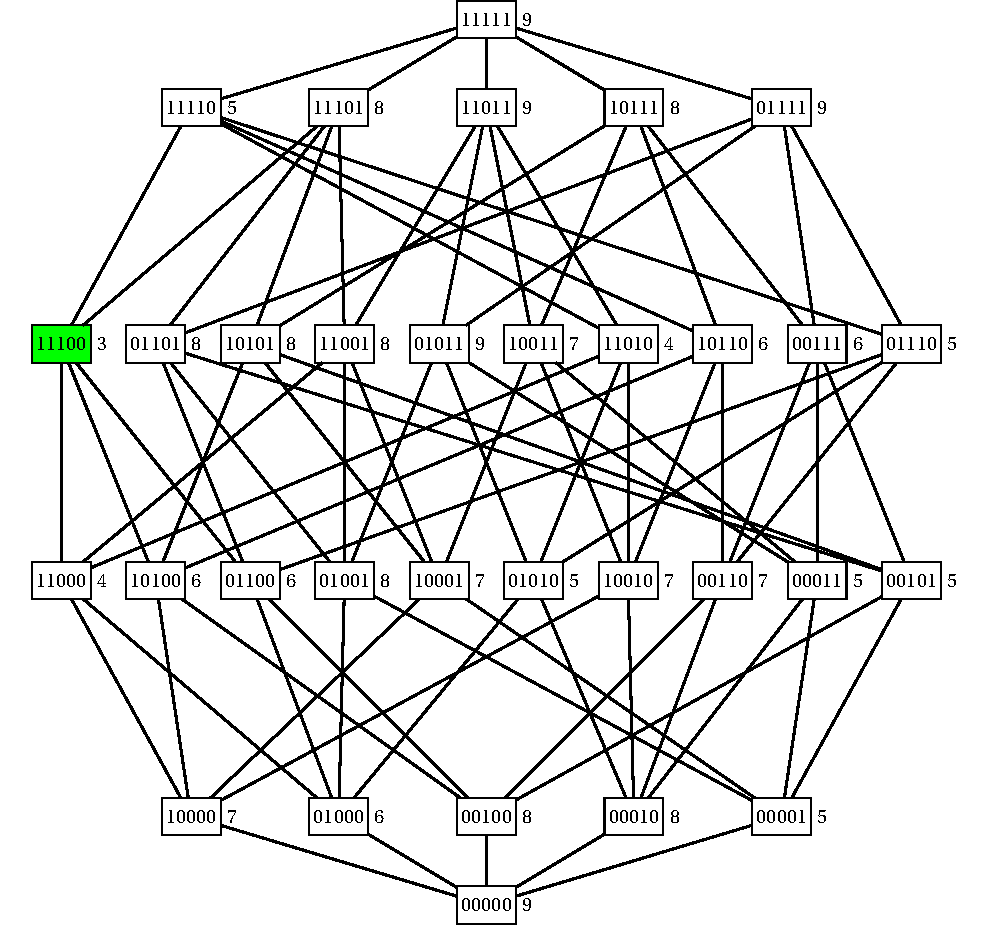
\includegraphics[clip=true, width=0.3\textwidth]{simulation/Boolean_lattice.pdf}
    }
     & \phantom{abcdefgh} &
    \subfigure {
        \label{fig:example:A}
        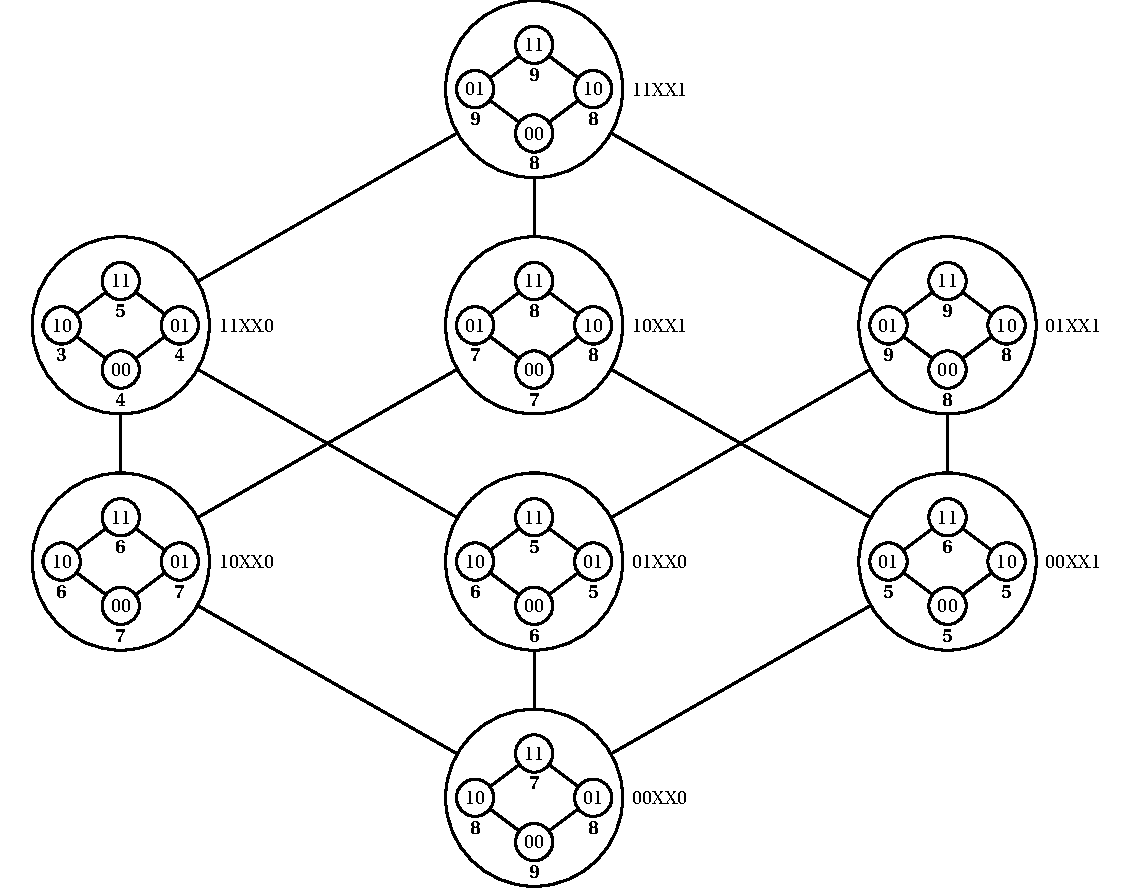
\includegraphics[clip=true, width=0.3\textwidth]{simulation/A.pdf}
    }
    \end{tabular}   
    \caption{An instance of the U-curve problem with $|S| = 5$ (left) and induced search space when the third and fourth elements are regarded as don't care (right).}
\end{figure}


    \begin{figure}[h]
    \begin{tabular}{l l c r r}
    \centering
    (a) &
    \subfigure {
        \label{fig:example:B}
        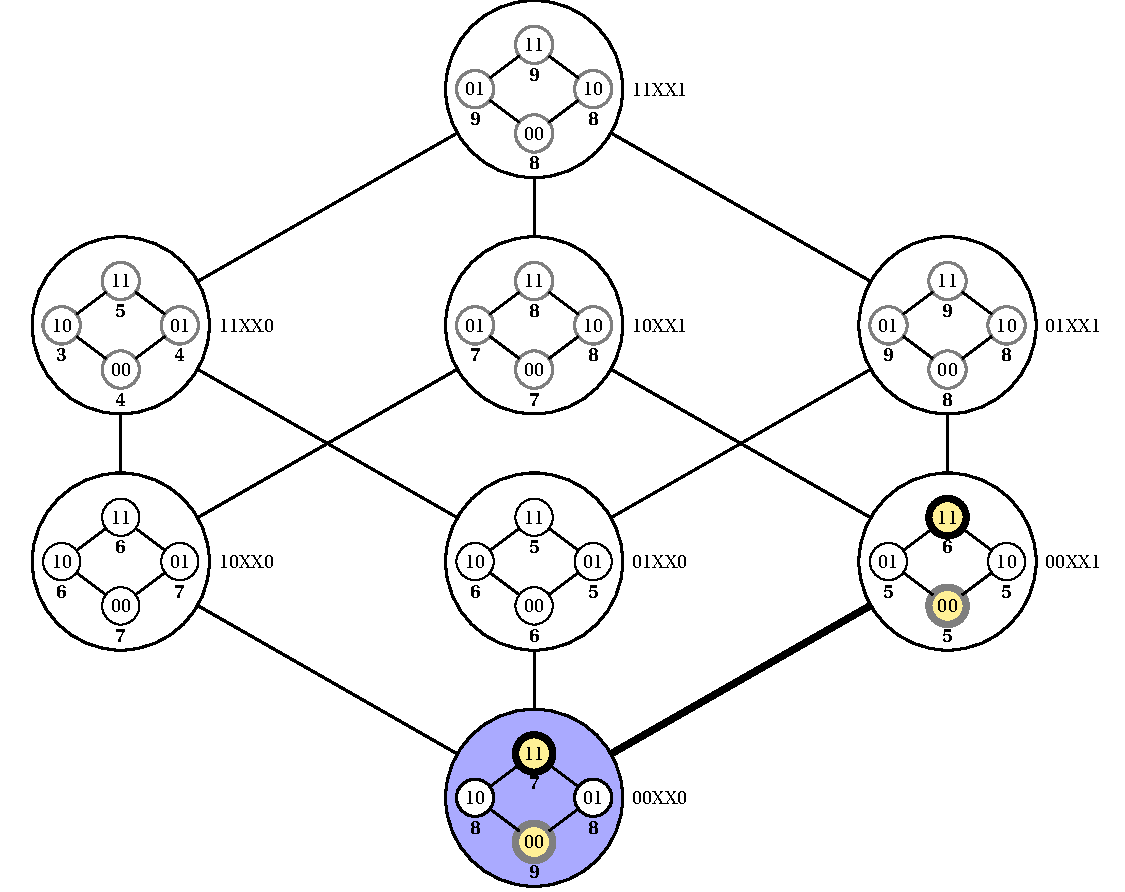
\includegraphics[ clip=true, width=0.29\textwidth]{simulation/B.pdf}
    }
    & \phantom{abcdefgh} &
    \subfigure {
        \label{fig:example:C}
        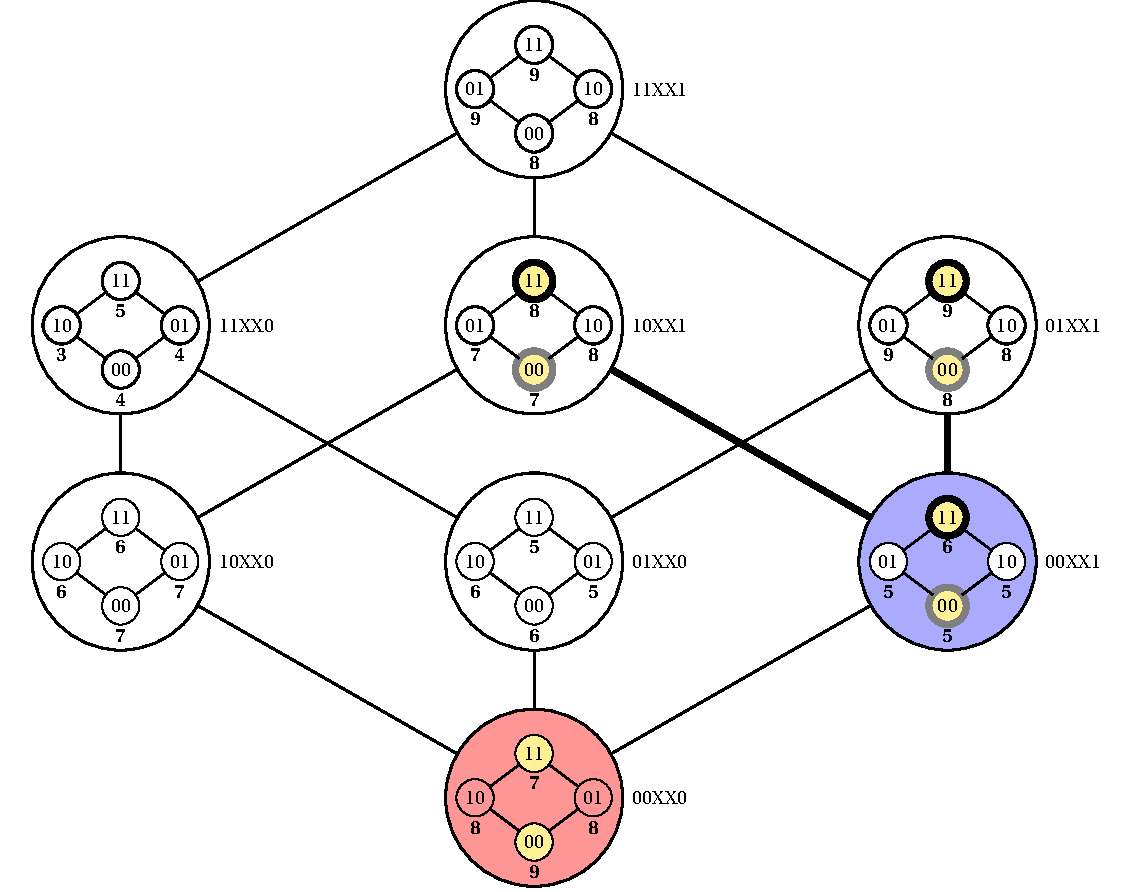
\includegraphics[clip=true, width=0.29\textwidth]{simulation/C.pdf}
    }
    & (b)
    \vspace*{.5cm} \\
    (c) &
    \subfigure {
        \label{fig:example:D}
        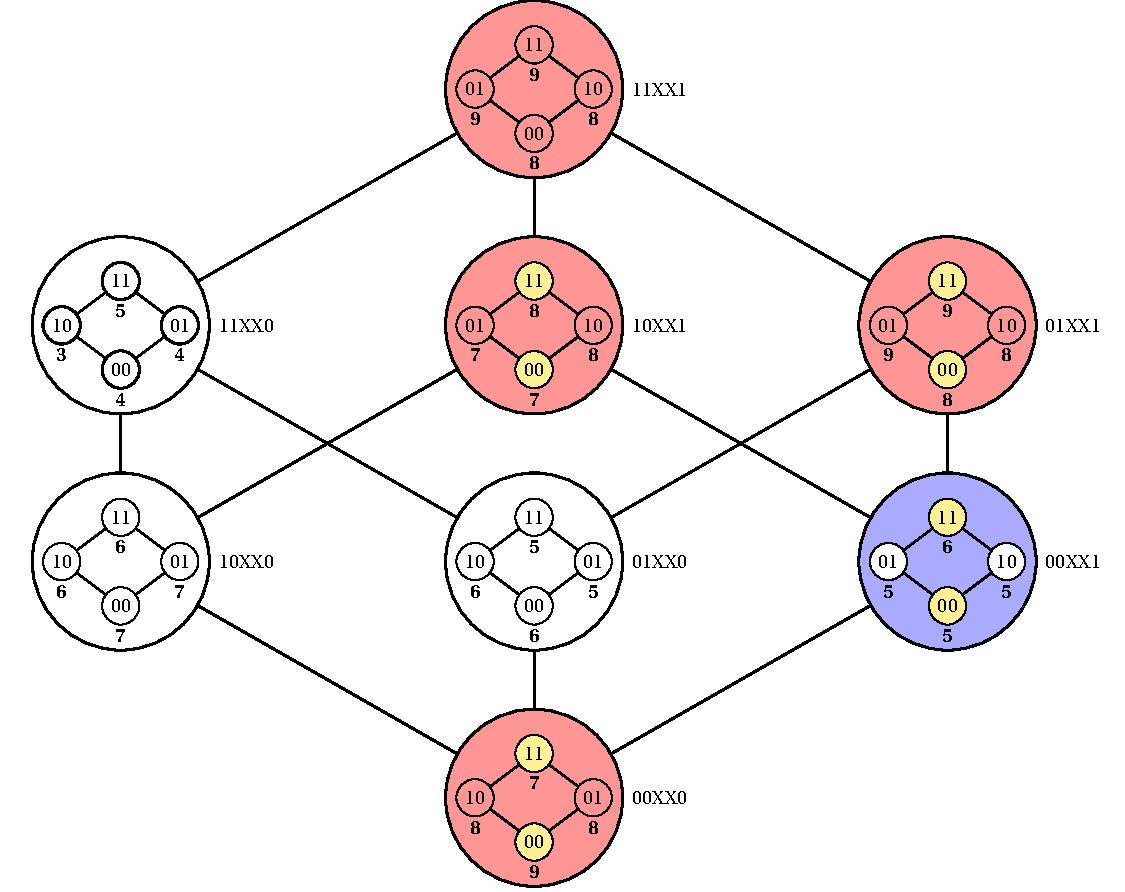
\includegraphics[ clip=true, width=0.29\textwidth]{simulation/D.pdf}
    }
    & \phantom{abcde} &
    \subfigure {
        \label{fig:example:E}
        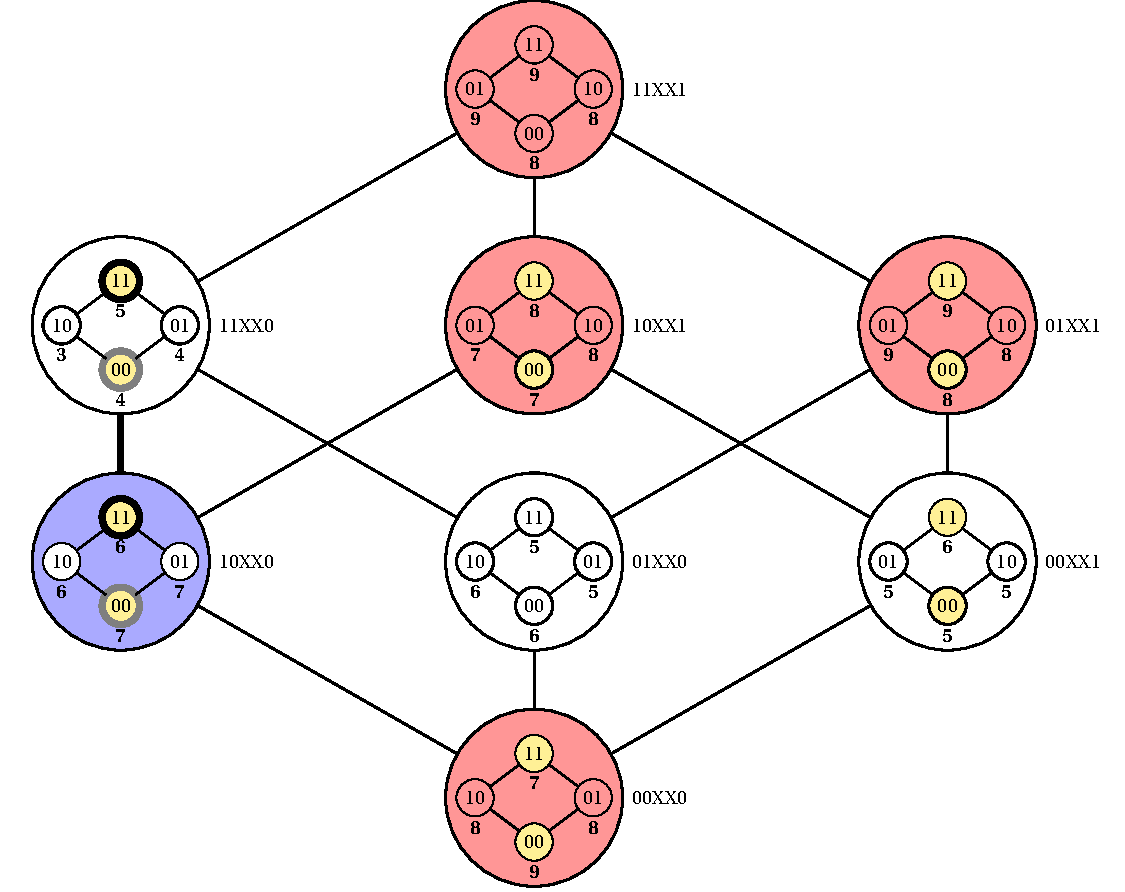
\includegraphics[clip=true, width=0.29\textwidth]{simulation/E.pdf}
    }
    & (d)
    \vspace*{.5cm} \\
    (e) &
    \subfigure {
        \label{fig:example:F}
        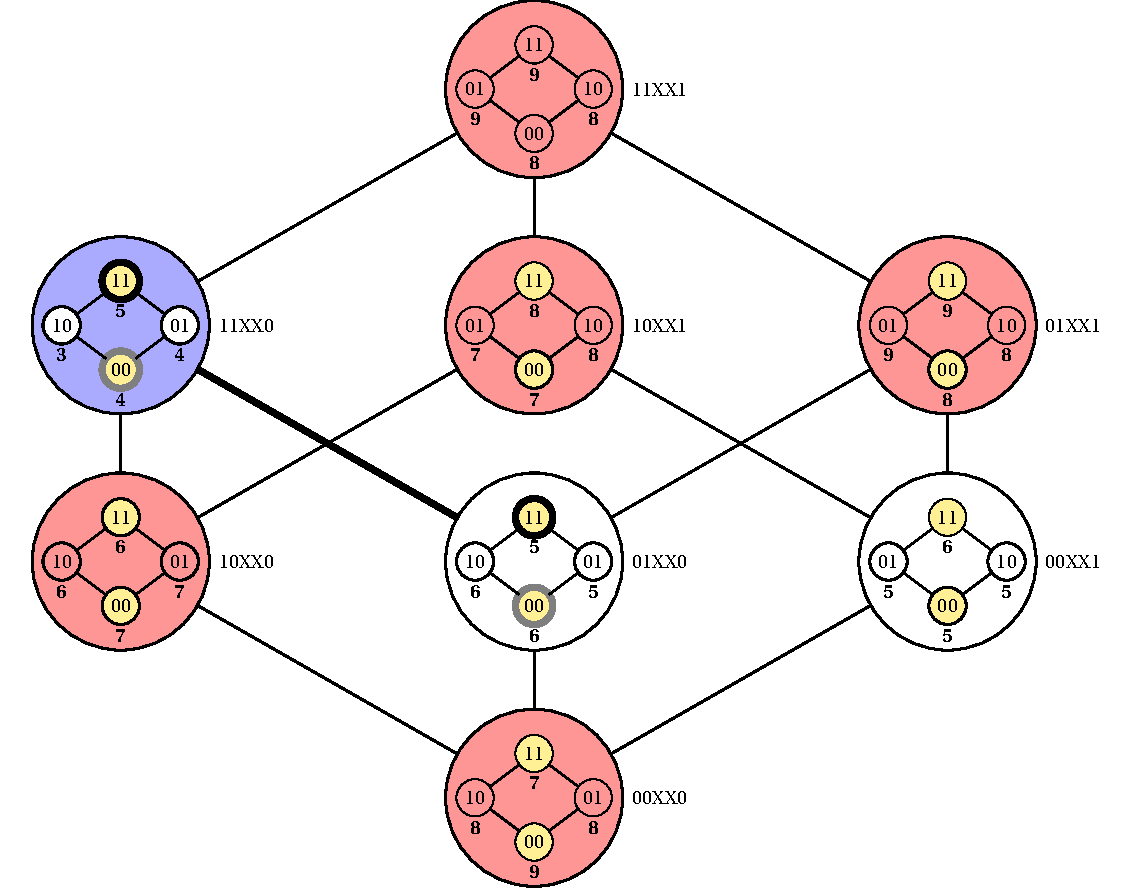
\includegraphics[ clip=true, width=0.29\textwidth]{simulation/F.pdf}
    }
    & \phantom{abcde} &
    \subfigure {
        \label{fig:example:G}
        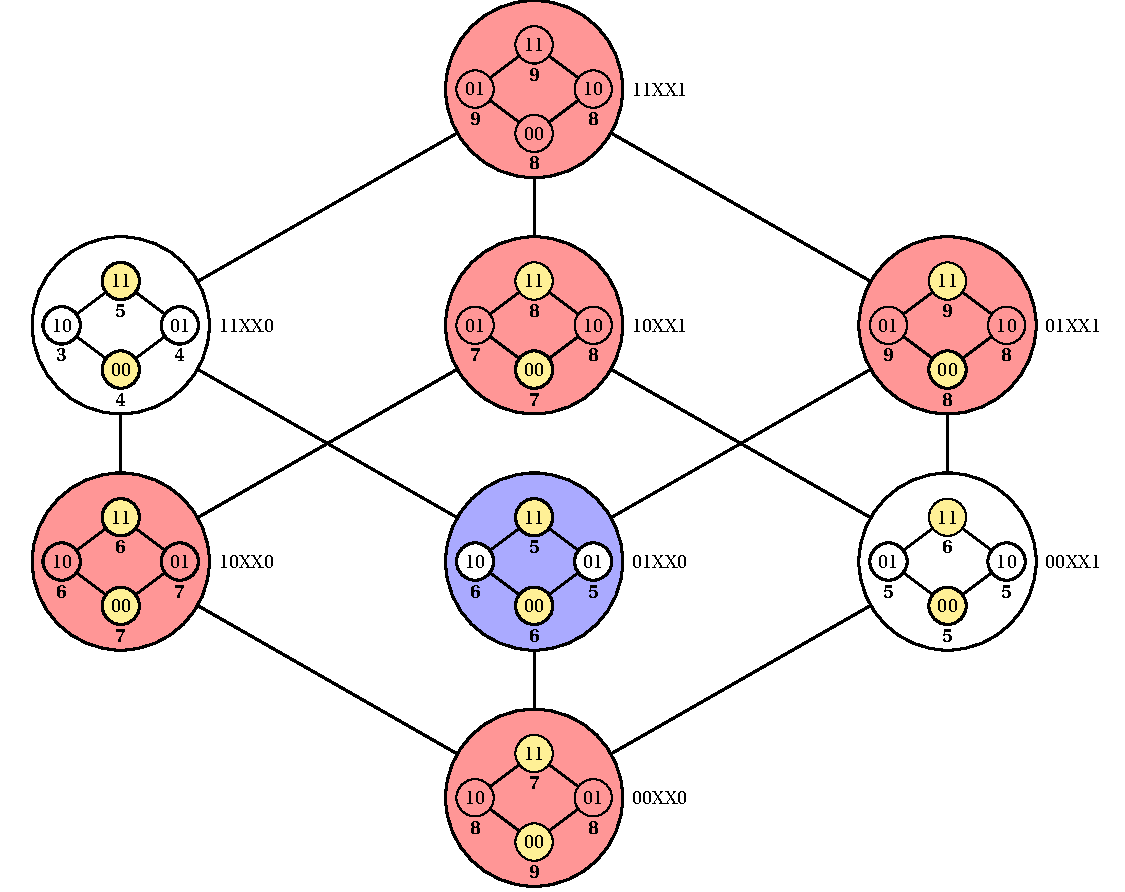
\includegraphics[clip=true, width=0.29\textwidth]{simulation/G.pdf}
    }
    & (f)
    \vspace*{.5cm} \\
    (g) &
    \subfigure {
        \label{fig:example:H}
        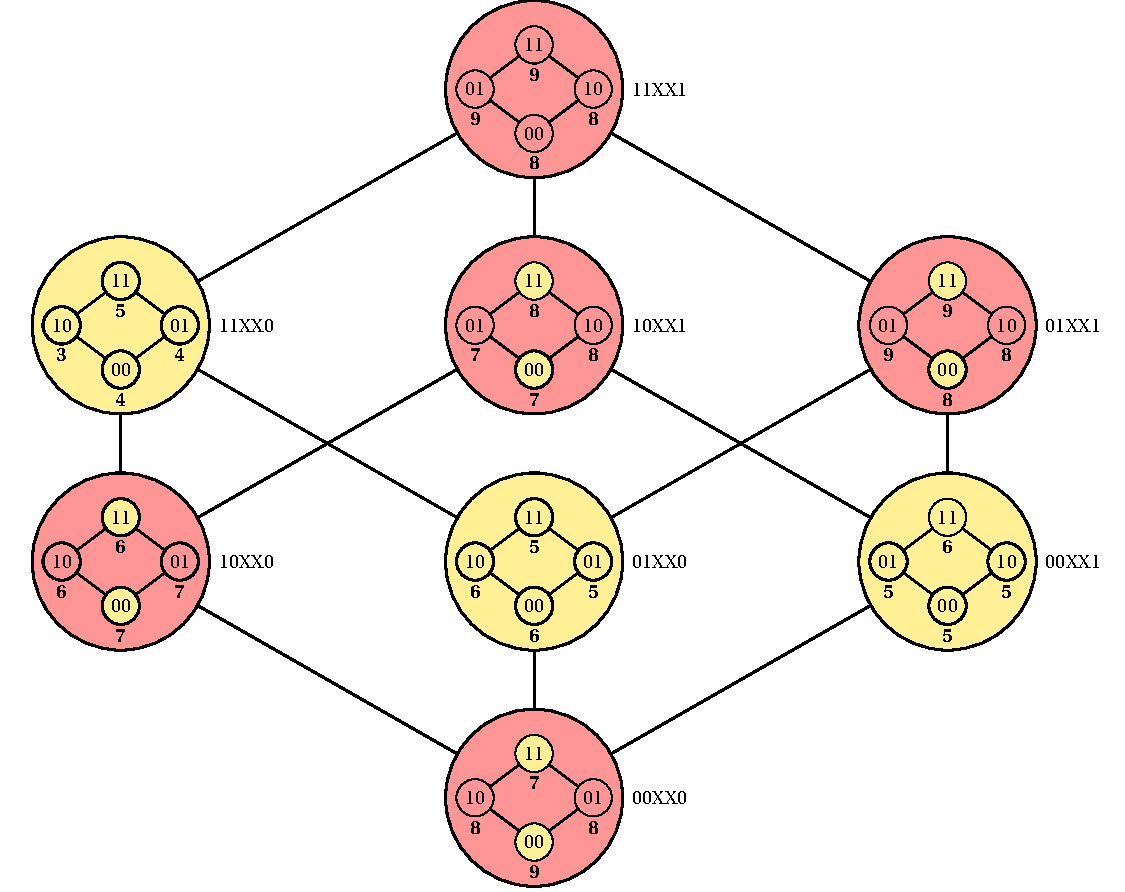
\includegraphics[ clip=true, width=0.29\textwidth]{simulation/H.pdf}
    }
    & \phantom{abcde} &
    \subfigure {
        \label{fig:example:I}
        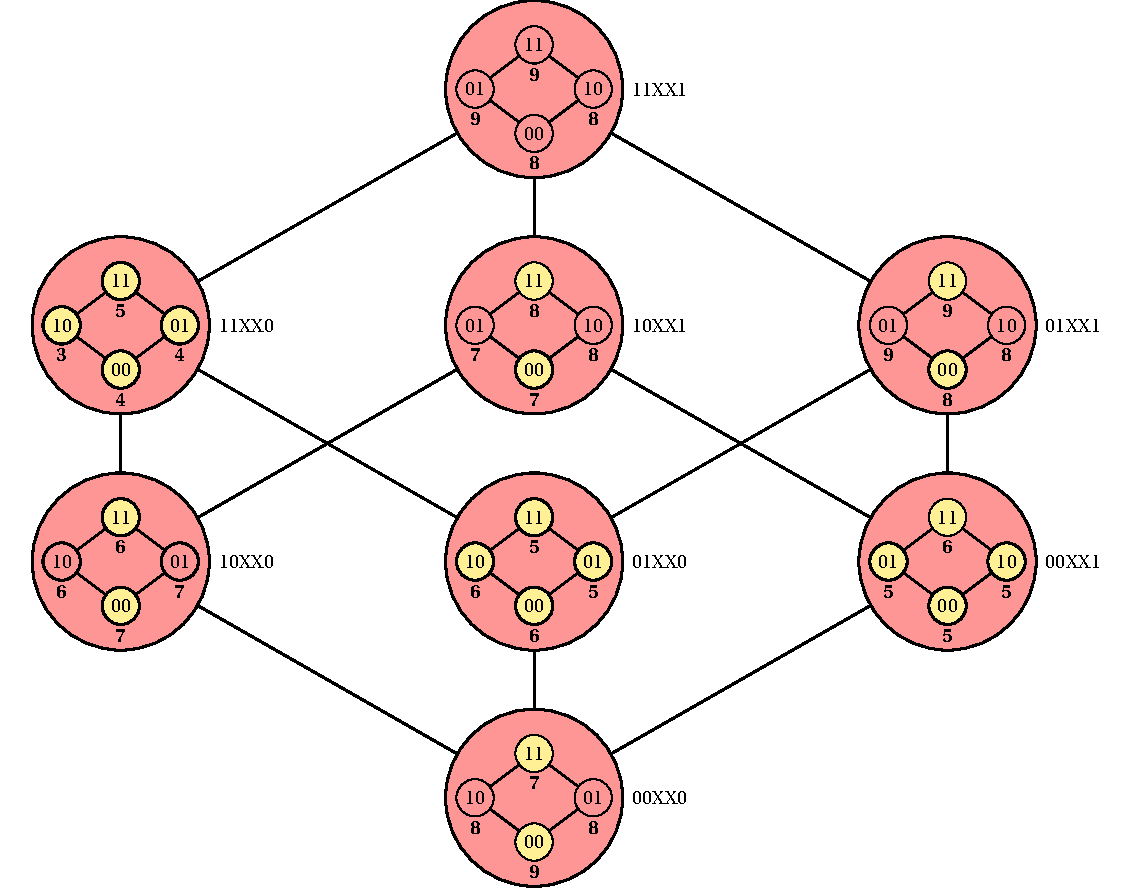
\includegraphics[clip=true, width=0.29\textwidth]{simulation/I.pdf}
    }
    & (h)
    \end{tabular}  
    \bigskip 
    \caption{Dynamics of the PUCS algorithm (Fig.~2(a)--(h)). In the outer lattice, blue, yellow and red colors mean a node being processed, solved or removed from the search space, respectively. In the inner lattice, yellow color on a given node means that the cost function was computed for its subset.}%
\end{figure}

\end{block}

\vfill 
\vspace*{.5cm}%
\begin{block}{Acknowledgements}%
% \insidecolumns{0.2}{2}%
% {\mycenteredimage{institutions/FAPESP.jpg}{1.1}}%
% {\mycenteredimage{institutions/capes.jpg}{1.2}}%
% {\mycenteredimage{institutions/CNPq.png}{1.5}}%

\vspace*{-1.5cm}%
\begin{figure}[h]
    \begin{tabular*}{0.7\textwidth}{c@{\extracolsep{\fill}}cc}
    \centering
    \subfigure {
        
\includegraphics[clip=true, width=0.2\textwidth]{institutions/FAPESP.jpg}
    }
    &
    \subfigure {
        
\includegraphics[clip=true, width=0.2\textwidth]{institutions/CNPq.png}
    }
    &
    \subfigure {
        
\includegraphics[clip=true, width=0.1\textwidth]{institutions/capes.jpg}
    }
    \end{tabular*}   
\end{figure}
\vspace*{1.5cm}%
\end{block}%
} % end \leftcolumn




\rightcolumn{              
\begin{block}{Results}%
\rightfigparagraph{figures/aproximation_like.png}{19}{15}{%
PUCS has two parameters: {\em p} and {\em l} determine 
the size of the outer lattice and the number 
of recursive calls before calling the base case solver, respectively. In our 
implementation, we were able to confirm our expectations that the
algorithm can find solutions as good as it possible (be optimal) as 
long as we increase the parameters {\em p} and {\em l}.
}%

\vspace{-1.5em}
\leftfigparagraph{qrcode_featsel.png}{4}{10}{
We used the {\em featsel} (\href{github.com/msreis/featsel}{github.com/msreis/featsel}), a C++ framework to implement and benchmark PUCS with other algorithms, such as Exhaustive Search (ES), Sequential Forward Selection (SFS) and 
Backward Feature Selection (BFS). These experiments were carried out in a 64-core, 256 GB RAM server (Fig.~3--4).
} % paragraph

\vspace{-1.5em}

\begin{figure}[h]
    \begin{tabular}{l r}
    \centering
    \subfigure {
        \label{fig:art_res:small:time}
        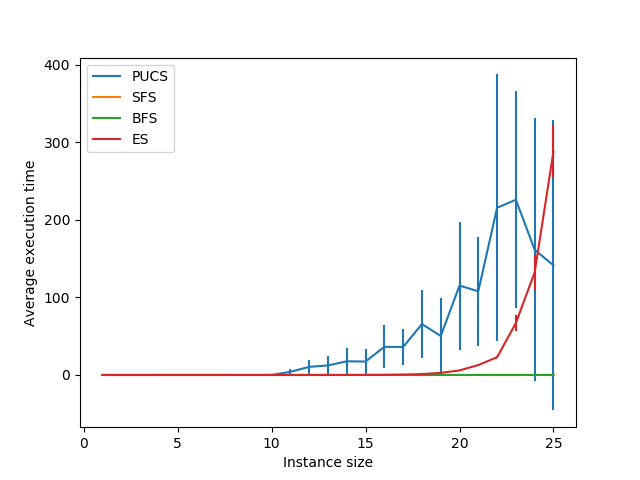
\includegraphics[clip=true, width=0.45\textwidth]{results/small_artificial_time.png}
    }
    &
    \subfigure {
        \label{fig:art_res:small:correctness}
        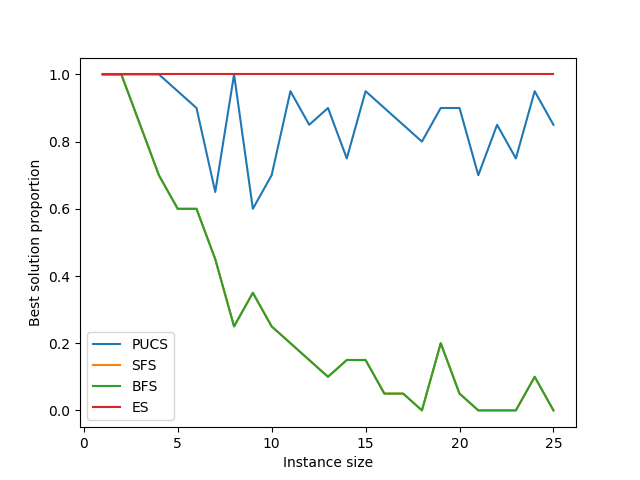
\includegraphics[clip=true, width=0.45\textwidth]{results/small_artificial_corr.png}
    } \\
    \subfigure {
        \label{fig:art_res:big:time}
        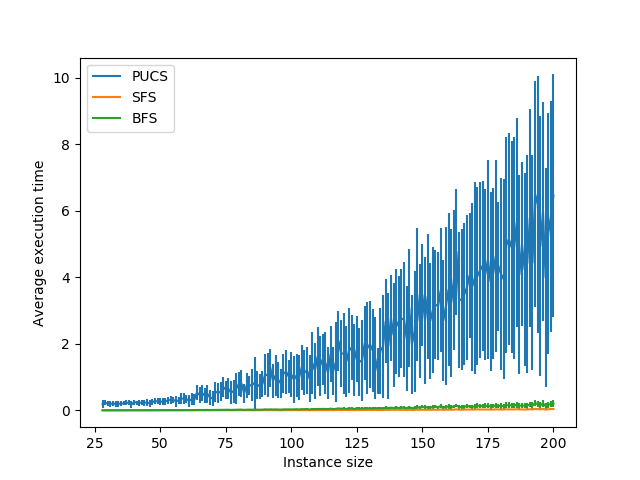
\includegraphics[clip=true, width=0.45\textwidth]{results/big_artificial_time.png}
    }
    &
    \subfigure {
        \label{fig:art_res:big:correctness}
        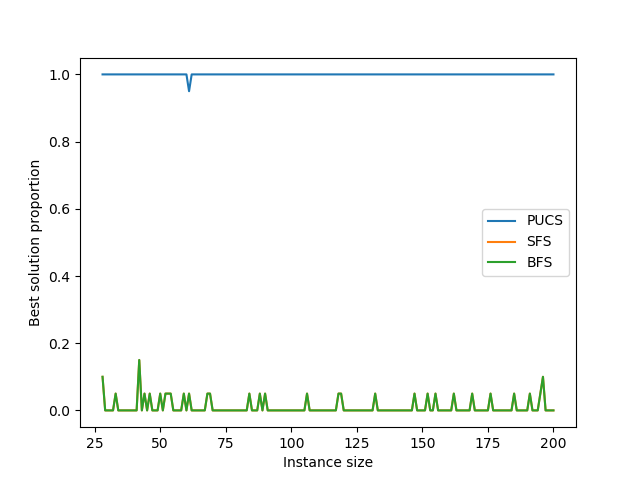
\includegraphics[clip=true, width=0.45\textwidth]{results/big_artificial_corr.png}
    }
    \end{tabular}   
    \caption{Average execution time and average number of times each algorithm found the best solution. For these instances, we used SFS to solve recursion base cases of the PUCS algorithm.}
    \label{fig:art_res} 
\end{figure}

\begin{figure}[h]
\centering
\begin{tabular}{l r}
    \centering
    \subfigure {
        \label{fig:art_res:small:time}
        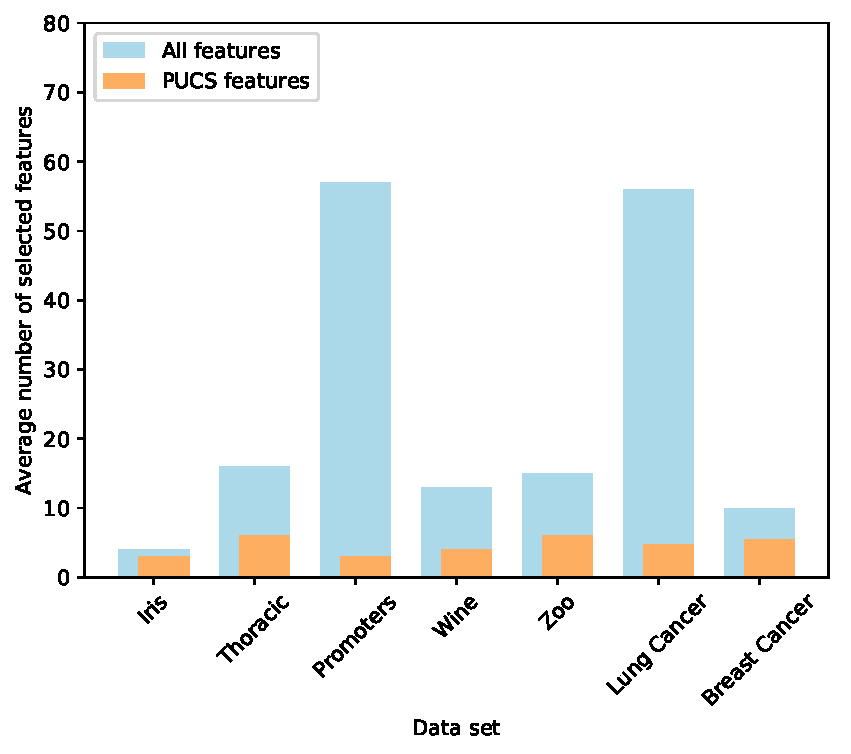
\includegraphics[clip=true, width=0.40\textwidth]{results/avg_features.pdf}
    }
    &
    \subfigure {
        \label{fig:art_res:small:correctness}
        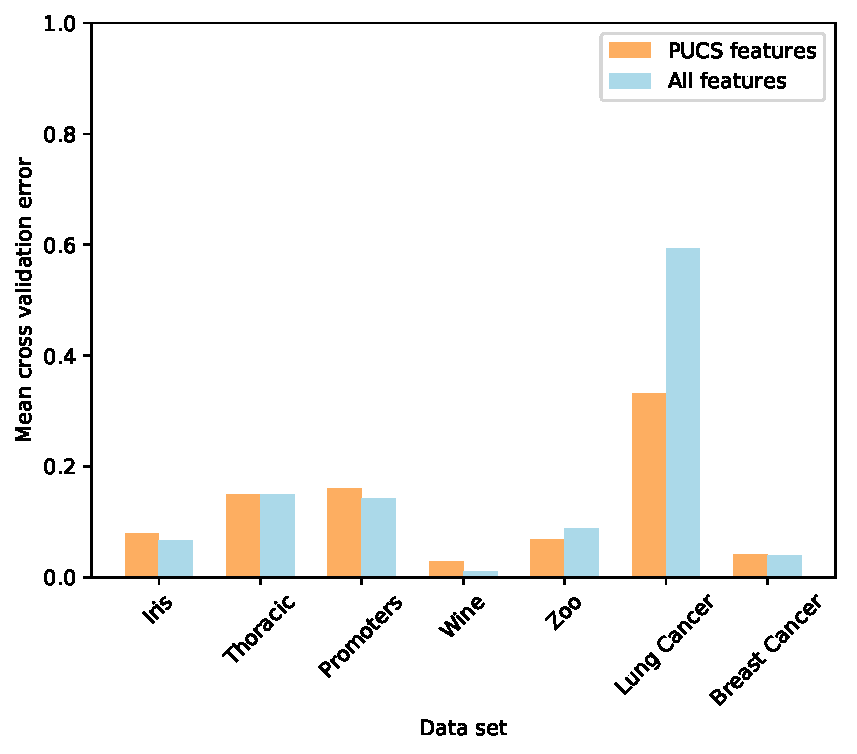
\includegraphics[clip=true, width=0.40\textwidth]{results/svm_error.pdf}
    }
\end{tabular}
\caption{Average number of features selected by PUCS and average cross-validation
    error when using these features to design SVM classifiers for some biological
    databases available at the UCI Machine Learning Repository.}
\label{fig:svm_error}
\end{figure}

\end{block}



%%%%%%%%%%%%%%%%%%%%%%%%%%%%%%%%%%%%%%%%%%%%%%%%%%%%%%%%%%%%%%%%%%%
\begin{block}{Conclusion}%
{
Results showed that PUCS has a better time performance than optimal solvers such as ES, and also can find better solutions than heuristics such as SFS and BFS. Future and ongoing work on this research line includes:
\begin{itemize}
    \bigskip
    \item{Design of new algorithms, especially ones that generalize the search space for poset forests;}
    \bigskip
    \item{Application of PUCS on the feature selection step in identification of cell signaling pathways.}
\end{itemize}
}
\end{block}
}% end of right column
\end{columns}
\end{frame}
\end{document}
